%%%%%%%%%%%%%%%%%%%%%%%%%%%%%%%%%%%%%%%%%
% Beamer Presentation
% LaTeX Template
% Version 1.0 (10/11/12)
%
% This template has been downloaded from:
% http://www.LaTeXTemplates.com
%
% License:
% CC BY-NC-SA 3.0 (http://creativecommons.org/licenses/by-nc-sa/3.0/)
%
%%%%%%%%%%%%%%%%%%%%%%%%%%%%%%%%%%%%%%%%%

%----------------------------------------------------------------------------------------
%	PACKAGES AND THEMES
%----------------------------------------------------------------------------------------

\documentclass{beamer}

\mode<presentation> {

% The Beamer class comes with a number of default slide themes
% which change the colors and layouts of slides. Below this is a list
% of all the themes, uncomment each in turn to see what they look like.

%\usetheme{default}
%\usetheme{AnnArbor}
%\usetheme{Antibes}
%\usetheme{Bergen}
%\usetheme{Berkeley}
%\usetheme{Berlin}
%\usetheme{Boadilla}
%\usetheme{CambridgeUS}
%\usetheme{Copenhagen}
%\usetheme{Darmstadt}
%\usetheme{Dresden}
%\usetheme{Frankfurt}
%\usetheme{Goettingen}
%\usetheme{Hannover}
%\usetheme{Ilmenau}
%\usetheme{JuanLesPins}
%\usetheme{Luebeck}
%\usetheme{Madrid}
%\usetheme{Malmoe}
%\usetheme{Marburg}
\usetheme{Montpellier}
%\usetheme{PaloAlto}
%\usetheme{Pittsburgh}
%\usetheme{Rochester}
%\usetheme{Singapore}
%\usetheme{Szeged}
%\usetheme{Warsaw}

% As well as themes, the Beamer class has a number of color themes
% for any slide theme. Uncomment each of these in turn to see how it
% changes the colors of your current slide theme.

%\usecolortheme{albatross}
%\usecolortheme{beaver}
%\usecolortheme{beetle}
%\usecolortheme{crane}
%\usecolortheme{dolphin}
%\usecolortheme{dove}
%\usecolortheme{fly}
%\usecolortheme{lily}
%\usecolortheme{orchid}
%\usecolortheme{rose}
%\usecolortheme{seagull}
%\usecolortheme{seahorse}
%\usecolortheme{whale}
%\usecolortheme{wolverine}

%\setbeamertemplate{footline} % To remove the footer line in all slides uncomment this line
%\setbeamertemplate{footline}[page number] % To replace the footer line in all slides with a simple slide count uncomment this line

%\setbeamertemplate{navigation symbols}{} % To remove the navigation symbols from the bottom of all slides uncomment this line
}

\usepackage{graphicx} % Allows including images
\usepackage{booktabs} % Allows the use of \toprule, \midrule and \bottomrule in tables

%----------------------------------------------------------------------------------------
%	TITLE PAGE
%----------------------------------------------------------------------------------------

\title[Mastering Metrics]{Understanding Metrics based on Mastering Metrics } % The short title appears at the bottom of every slide, the full title is only on the title page

\author{Corinna Birner \& Max M{\"u}ller} % Your name
\institute[JMU] % Your institution as it will appear on the bottom of every slide, may be shorthand to save space
{University of W{\"u}rzburg }\\ % Your institution for the title page
\medskip
\textit{{corinna.birner@stud-mail.uni-wuerzburg.de 
max.mueller@stud-mail.uni-wuerzburg.de} % Your email address
}
\date{\today} % Date, can be changed to a custom date

%------------------------------------------------
\begin{document}

\begin{frame}
\titlepage % Print the title page as the first slide
\end{frame}

%------------------------------------------------
\begin{frame}
\begin{center}
\textbf\Huge{Chapter 4: Regression Discontinuity Designs}
\end{center}
\end{frame}

%------------------------------------------------
\begin{frame}
\frametitle{Overview} % Table of contents slide, comment this block out to remove it
Today we will continue our journey on the path from cause to effect. Therefore, we will discuss regression discontinuity (RD) designs as one possible way of finding causal relations in our data. Our topics will be the following:

\tableofcontents % Throughout your presentation, if you choose to use \section{} and \subsection{} commands, these will automatically be printed on this slide as an overview of your presentation
\end{frame}

%----------------------------------------------------------------------------------------
%	PRESENTATION SLIDES
%----------------------------------------------------------------------------------------

%------------------------------------------------
\section{Minimum Legal Drinking Age}

\begin{frame}
\frametitle{Whats a RDD?}
\begin{itemize}
	\item We use rules, even arbitrary ones, to exploit certain circumstances
	\item E.g. The State of California limits elementary school class size to 32 students; 33 is one too many.
	\item	32 in that case would be our threshold.
	\item Regression discontinuity (RD) designs exploit discontinuities in policy assignment. 
	\item Assume that units on different sides of the discontinuity are similar. Their treatment status differs only because of the institutional setup, and therefore differences in outcomes can be attributed to the different treatment status.
\end{itemize}
\end{frame}

%------------------------------------------------
%------------------------------------------------
% Sections can be created in order to organize your presentation into discrete blocks, all sections and subsections are automatically printed in the table of contents as an overview of the talk

%------------------------------------------------

%\subsection{Even more Nonsense} % A subsection can be created just before a set of slides with a common theme to further break down your presentation into chunks


%------------------------------------------------
\begin{frame}
\frametitle{Minimum Legal Drinking Age}
\begin{itemize}
	\item Lets take a look at one of the most important thresholds for young americans: If they are over 21, they can drink legally
	\item This experiment emerges from the fact that a small change in age (measured in months or even days) generates a big change in legal access. 
	\item The difference a day makes can be seen in Figure 4.1, which plots the relationship between birthdays and funerals.
	\item So we could assume that the individuals only differ in their legal drinking access one day before and one day after turning 21.
\end{itemize}

\end{frame}
%------------------------------------------------
\begin{frame}
\frametitle{Minimum Legal Drinking Age}
\begin{columns}
\column{.5\textwidth}
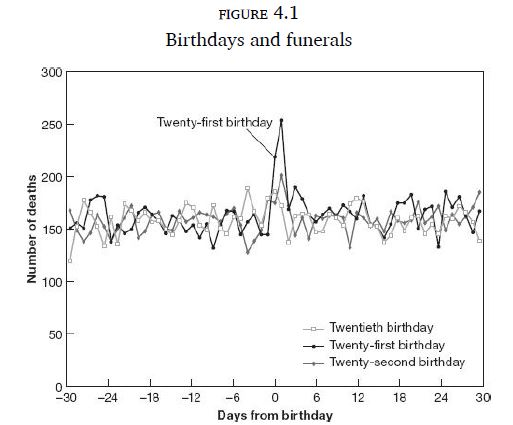
\includegraphics[width=6cm,height=6.5cm,keepaspectratio]{Figure 4.1} 

\column{.45\textwidth}
\begin{itemize}
	\item Shows the number of deaths among Americans aged 20–22 between 1997 and 2003. 
	\item Deaths here are plotted by day, relative to birthdays, which are labeled as day 0.
\end{itemize}

\end{columns}
\end{frame}
%------------------------------------------------
\begin{frame}
\frametitle{Birthday Comparisons}
\begin{itemize}
\item Mortality risk shoots up on and immediately following a twenty-first birthday
\item Does not happen around the twentieth and twenty-second birthdays
\item So there has to be something special around the 21st Birthday that influences death rates.
\end{itemize}
\end{frame}
%------------------------------------------------
\begin{frame}
\frametitle{Cut-Off}
\begin{columns}
\column{.5\textwidth}
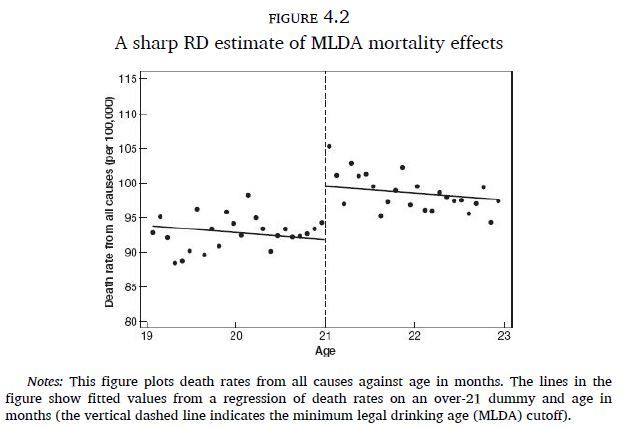
\includegraphics[width=6cm,height=6.5cm,keepaspectratio]{Figure 4.2} 

\column{.45\textwidth}
\begin{itemize}
	\item This figure plots death rates (measured as deaths per 100,000 persons per year) by month of age (defined as 30- day intervals), centered around the twenty-first birthday. 
	\item The X-axis extends 2 years in either direction, and each dot in the figure is the death rate in one monthly interval.
\end{itemize}

\end{columns}
\end{frame}

%------------------------------------------------
\begin{frame}
\frametitle{Cut-Off}
\begin{itemize}
	\item Few rates to the left of the age-21 cutoff are above 95. 
	\item At ages over 21, however, death rates shift up, and few of those to the right of the age-21 cutoff are below 95.
	\item Extrapolating the trend line drawn to the left of the cutoff, we might have expected an age-21 death rate of about 92, while the trend line to the right of 21 starts markedly higher, at around 99.
	\item Jump in trend lines at age 21 illustrates the subject of this chapter, regression discontinuity designs.
\end{itemize}
\end{frame}
%------------------------------------------------
\begin{frame}
\frametitle{The Treatment Variable}
\begin{itemize}
	\item RD is based on the idea that rigid rules create valuable experiments.
	\item Causal question here is the effect of legal access to alcohol on death rates. 
	\item The treatment variable in this case can be written as: 
	$$D_a = \left\{
	\begin{align}
1~ if~ a~ \geq ~21 \\
0~ if~ a~ < ~21		
	\end{align}
	$$
\end{itemize}

\end{frame}
%------------------------------------------------
\begin{frame}
\frametitle{Features of RD Designs}
\begin{itemize}
	\item This representation highlights two signal features of RD designs:
	\begin{itemize}
		\item[\bullet] Treatment status is a deterministic function of a, so that once we know a, we know $D_a$.
		\item[\bullet] Treatment status is a discontinuous function of a, because no matter how close a gets to the cutoff, $D_a$ remains unchanged until the cutoff is reached.
	\end{itemize}
	\item The variable that determines treatment, age in this case, is called the running variable.
	\item 2	Kinds of RDD´s:
\begin{itemize}
		\item[\bullet] Sharp RD designs: Treatment switches cleanly off or on as the running variable passes a cutoff.
		\item[\bullet] Fuzzy RD: The probability or intensity of treatment jumps at a cutoff.
	\end{itemize}
\end{itemize}
\end{frame}
%------------------------------------------------
\begin{frame}
\frametitle{Regression in RD}
\begin{itemize}
	\item In this case it’s a sharp RD, because the MLDA is a sharp function of age
	\item Mortality clearly changes with the running variable, a, for reasons unrelated to the MLDA.
	\item A simple RD analysis of the MLDA estimates causal effects using a regression like: 
	$$\bar{M}_a=\alpha + \rho D_a + \gamma a + \epsilon_a$$
	\item $\bar{M}_a$ is the death rate in month a, includes the treatment dummy, $D_a$, and linear control for age in months.
\end{itemize}
\end{frame}
%------------------------------------------------
\section{Cut off difference} 
\begin{frame}
\frametitle{The Regression Framework}
\begin{itemize}
	\item Fitted values from this regression produce the lines drawn in Figure 4.2. 
	\item The negative slope, captured by $\gamma$, reflects smoothly declining death rates among young people as they mature. 
	\item The parameter $\rho$ captures the jump in deaths at age 21.
	\item This Regression generates an estimate of $\rho$ equal to 7.7. 
	\item When cast against average death rates of around 95, this estimate indicates a substantial increase in risk at the MLDA cutoff.
\end{itemize}
	
\end{frame}
%------------------------------------------------
\begin{frame}
\frametitle{Control for other Things?}

\begin{itemize}
	\item Should we not control for other things? 
	\item The OVB formula tells us that the difference between the estimate of $\rho$ in this short regression and the results any longer regression might produce depend on the correlation between variables added to the long regression and $D_a$. 
	\item But: $D_a$ is determined solely by a. 
	\item So we can be sure that no OVB afflicts this short regression.
\end{itemize}

\end{frame}
%------------------------------------------------
\begin{frame}
\frametitle{Regression in RD}
\begin{itemize}
	\item Although treatment isn´t randomly assigned, we know where it comes from. 
	\item Treatment is determined by the running variable.
	\item RD uses regression methods to estimate causal effects, but we don’t need matching and regression strategies which are based on treatment-control comparisons conditional on covariate values.
	\item In this case, only the running variable, the changes in access to alcohol for young people, matters.
\end{itemize}

\end{frame}

%------------------------------------------------
\begin{frame}
\frametitle{Problem of Nonlinearity}
\begin{columns}
\column{.5\textwidth}
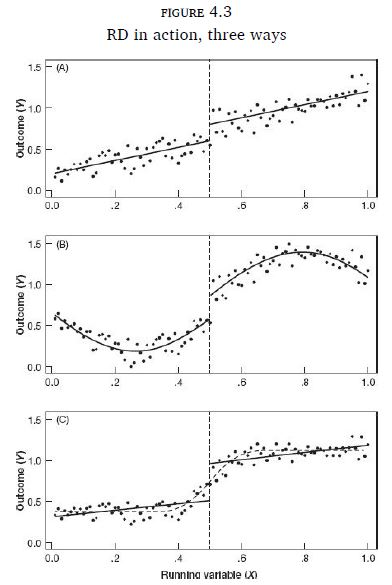
\includegraphics[width=6cm,height=6.5cm,keepaspectratio]{Figure 4.3} 

\column{.45\textwidth}
\begin{itemize}
	\item Panel A: relationship between the running variable (X) and the outcome (Y) is linear, clear jump at the cutoff 
	\item Panel B similar, the relationship between average Y and X is nonlinear.
	\item Panel C shows nonlinearity mistaken for a discontinuity.
\end{itemize}
\end{columns}	
\end{frame}
%------------------------------------------------
\begin{frame}
\frametitle{Public-Private Face-Off}

\begin{itemize}
	\item Two strategies reduce the likelihood of RD mistakes
	\item First: Nonlinear modeling strategy
	\item Nonlinearities in an RD framework are typically modeled using polynomial functions of the running variable.
	\item We modify our regression, if we think our model is non linear.
\end{itemize}

\end{frame}

%------------------------------------------------
\begin{frame}
\frametitle{Modify the regression}
\begin{itemize}
	\item Figure 4.2: possibility of mild curvature in the relationship Between ${M}_a$ and a, at least for the points to the right of the cutoff. 
	\item Extension that captures this curvature uses quadratic instead of linear control for the running variable. 
	\item The RD model with quadratic running variable control becomes:
	$$\bar{M}_a=\alpha + \rho D_a + \gamma_1 a +\gamma_2 a^2 + \epsilon_a $$
	\item Where $\gamma_1 a + \gamma_2 a^2$ is a quadratic function of age

\end{itemize}

\end{frame}

%------------------------------------------------
\begin{frame}
\frametitle{Modification}
\begin{itemize}
	\item A related modification allows for different running variable Coefficients to the left and right of the cutoff.
	\item To make the model with interactions easier to interpret, we center the running variable by subtracting the cutoff, $a_0$. 
	\item Replacing a by $a - a_0$ (here, $a_0$ = 21), and adding an interaction term, ($a - a_0$)$D_a$, the RD model becomes:
$$\bar{M}_a=\alpha + \rho D_a + \gamma (a - a_0) + \delta[(a - a_0)D_a] + \epsilon_a $$
\end{itemize}

\end{frame}
%------------------------------------------------
\begin{frame}
\frametitle{Model with interaction terms}
\begin{itemize}
	\item An implication of the model with interaction terms is that away from the $a_0$ cutoff, the MLDA treatment effect is given by $\rho + \delta(a - a0)$.
	\item Estimates away from the cutoff constitute a bold extrapolation, there is no world in which drinking is illegal with 24 or legal with 12.
	\item It seems reasonable to say that those just under 21 provide a good counterfactual comparison for those just over 21. 
	\item So estimates of the parameter $\rho$ (the causal effect right at the cutoff) are most reliable.
\end{itemize}

\end{frame}
%------------------------------------------------
\begin{frame}
\frametitle{Comparison of functions}
\begin{columns}
\column{.5\textwidth}
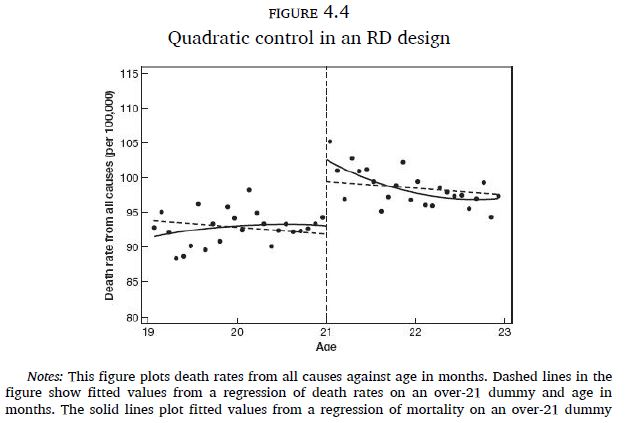
\includegraphics[width=6cm,height=6.5cm,keepaspectratio]{Figure 4.4} 

\column{.45\textwidth}
\begin{itemize}
	\item Curvature, mildly concave to the left of age 21 and convex thereafter. 
	\item This model generates a larger estimate of the MLDA effect at the cutoff than does a linear model, 9.5 deaths per 100,000.
\end{itemize}
\end{columns}	
\end{frame}
%------------------------------------------------
\begin{frame}
\frametitle{Comparison}
\begin{itemize}
	\item Comparison: more elaborate model seems to give a better fit than the simple model: Death rates jump sharply at age 21, but then recover somewhat in the first few months after a twenty-first birthday.
	\item Which version is better?: simple RD model seems flexible enough to capture effects right at the cutoff.
	\item But: The fancier version fits the spike in death rates near twenty-first birthdays, while also capturing the subsequent partial recovery in death rates.
	\item How convincing is the argument that the jump in Figure 4.4 is indeed due to drinking?
	\item few people die from alcohol poisoning alone, more deaths from alcohol-related diseases
	\item But: alcohol is closely tied to motor vehicle accidents (MVA), the number-one killer of young people.
\end{itemize}

\end{frame}
%------------------------------------------------
\begin{frame}
\frametitle{Estimates}
\begin{columns}
\column{.5\textwidth}
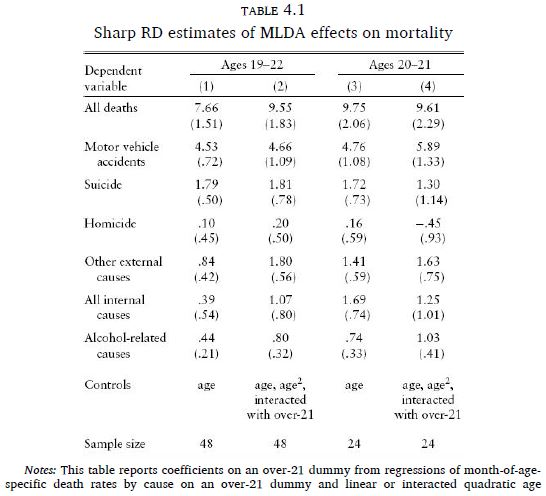
\includegraphics[width=6cm,height=6.5cm,keepaspectratio]{Table 4.1} 

\column{.45\textwidth}
\begin{itemize}
	\item second row reveals strong effects of legal drinking on MVA fatalities, effects large enough to account for most of the excess deaths related to the MLDA.
	\item Effects from direct alcohol poisoning appear to be modest
\end{itemize}
\end{columns}	

\end{frame}

%------------------------------------------------

\begin{frame}
\frametitle{Alcohol causes death?}
\newline 
\begin{itemize}
	\item Table 4.1 supports the MLDA story, showing clear effects for causes most likely attributable to alcohol but little evidence of an increase due to internal causes.
	\item Not much of a jump in deaths due to internal causes, while the standard errors suggest that the small jump in internal deaths is likely due to chance.
	\item straightforward regression estimation is also called parametric RD.

\end{itemize}

\end{frame}

%---------------------------------------------------

\begin{frame}
\frametitle{Close to the boundary}
\begin{itemize}
	\item Second RD strategy: Nonparametric RD for the small set of points close to the boundary, nonlinear trends need not concern us at all. 
	\item Suggests an approach that compares averages in a narrow window just to the left and just to the right of the cutoff. 
	\item A drawback here is that if the window is very narrow, there are few observations left, meaning the resulting estimates are likely to be too imprecise to be useful.
\end{itemize}

\end{frame}

%---------------------------------------------------
\begin{frame}
\frametitle{Nonparametric RD}
\begin{itemize}
	\item Nonparametric RD amounts to estimating the former regression in a narrow window around the cutoff.
	\begin{*flalign}
\begin{flushleft}
~M_a=\alpha + \rho D_a + \gamma a  + \epsilon_a; \\
~in~ a ~sample~ such~ that~ a_0 - b \leq a \leq a_0 +b
\end{flushleft}
	\end{*flalign}
	\item The parameter b describes the width of the window and is called a bandwidth.
	\item Table 4.1 can be seen as nonparametric RD with a bandwidth equal to 2 years of age for the estimates reported in columns (1) and (2) and a bandwidth half as large (that is, including only ages 20–21 instead of 19–22 for the estimates shown in columns (3) and (4). 


\end{itemize}
\end{frame}
%---------------------------------------------------

\begin{frame}
\frametitle{Parametric vs. Non-parametric approach}
\begin{itemize}
	\item Parametric tests: assume underlying statistical distributions (funtional form) in the data - Therefore, several conditions of validity must be met so that the result of a parametric test is reliable.
	\item Non-parametric: Do not rely on any distribution and can always be applied.
	\item We need to be aware of the assumptions associated with a parametric procedure.
	\item E.g. in parametric tests, we assume Effect homogeneity, which means that a added control variable has the same effect for every part of the distribution. (Treated individual)
	
\end{itemize}
\end{frame}

%---------------------------------------------------
%bis hier hin aktuell von Max_finished
%---------------------------------------------------
%Corinna neu
%---------------------------------------------------
%---------------------------------------------------
\begin{frame}
\frametitle{Peer effects in exam schools}
\begin{itemize}
\item In bigger cities in the US, the public school systems include a few very selective exam schools
\item in Boston for example the John D. O’Bryant School, Boston Latin Academy, Boston Latin School
\item the exam schools choose students based on competitive admission tests
\item What is the effect of going to such an exam school?
\item Problem: Peer Effect: intelligent students benefit from studying with intelligent students
\end{itemize}
\end{frame}

%---------------------------------------------------
\begin{frame}
\frametitle{Exam Schools - application for an RDD?}
\begin{itemize}
\item the discrete nature of exam school admission policies creates a natural experiment
\item among applicants with scores close to admission cutoffs, whether an applicant falls to the left ot the right of the cutoff might be as good as randomly assigned
\item with the sharp cut-off, it could be a good application for an RD
\item But: some admitted student choose to go elsewhere while many of the rejected at one exam school end up at another
\item When discontiniuities change treatment probablities or average characteristics instead of flicking a simple on-off switch, the RD design is said to be fuzzy
\end{itemize}
\end{frame}

%---------------------------------------------------

%---------------------------------------------------
\begin{frame}
\frametitle{The exam school treatment}
\begin{columns}
\column{.5\textwidth}
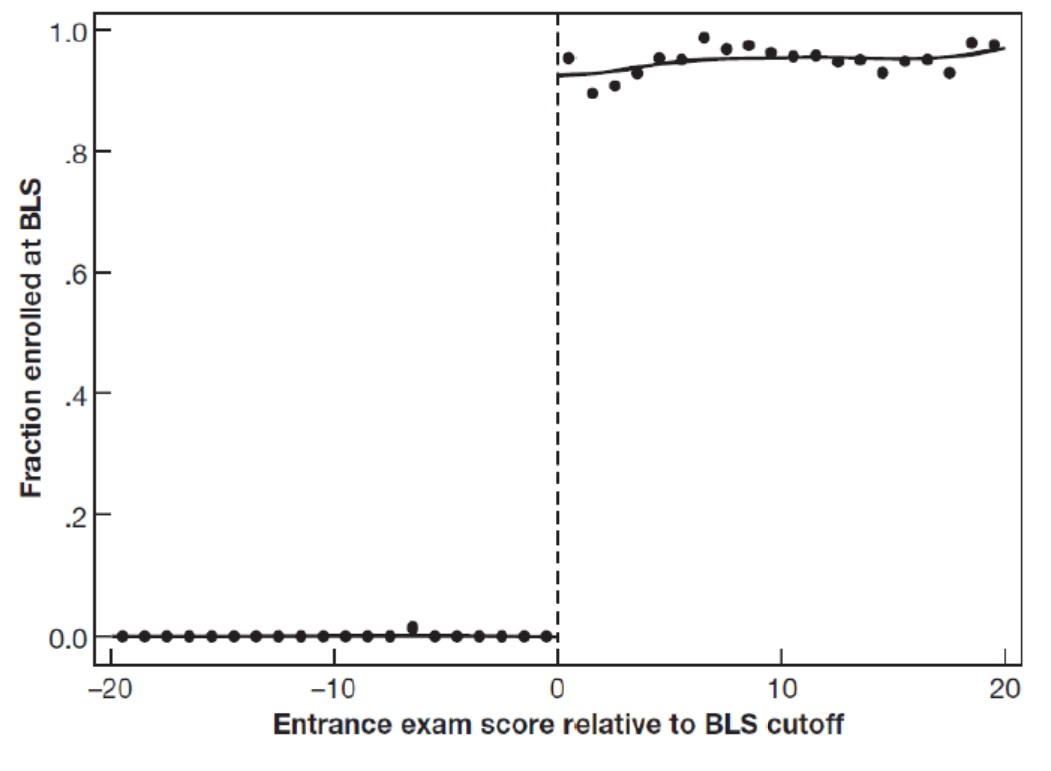
\includegraphics[width=6cm,height=6.5cm,keepaspectratio]{Figure 4.6} 

\column{.45\textwidth}
\begin{itemize}
	\item BLS is the most prestigious exam school
	\item sample for the figures are applicants for BLS with score close to the entrance cutoff
	\item where do applicants who miss the cutoff go?
	
\end{itemize}
\end{columns}	
\end{frame}

%---------------------------------------------------
\begin{frame}
\frametitle{The exam school treatment}
\begin{columns}
\column{.5\textwidth}
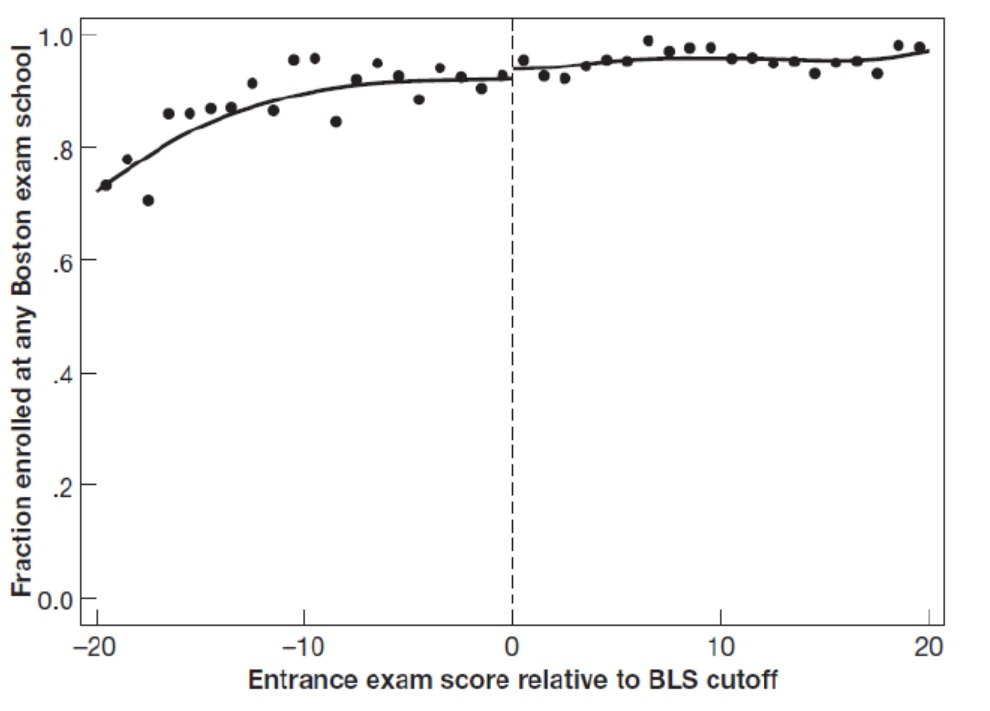
\includegraphics[width=6cm,height=6.5cm,keepaspectratio]{Figure 4.7} 

\column{.45\textwidth}
\begin{itemize}
	\item Figure shows enrollment at any Boston exam school
	\item most students that miss BLS cut-off end up at another exam school
	\item Can we therefore only compare two schools?
	
\end{itemize}
\end{columns}	
\end{frame}
%---------------------------------------------------
\begin{frame}
\frametitle{The exam school treatment}
\begin{columns}
\column{.5\textwidth}
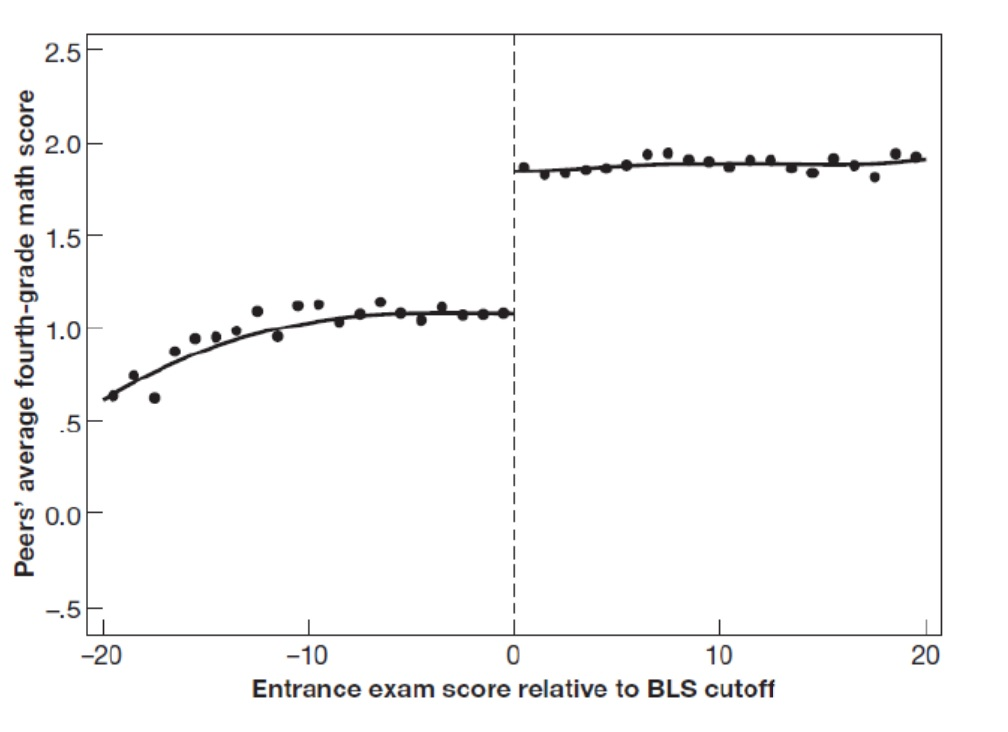
\includegraphics[width=6cm,height=6.5cm,keepaspectratio]{Figure 4.8} 

\column{.45\textwidth}
\begin{itemize}
	\item one controversial question in education research are peer effects
	\item to what extend does the quality of fellow students contribute the own success?
	
\end{itemize}
\end{columns}	
\end{frame}

%---------------------------------------------------
\begin{frame}
\frametitle{The exam school treatment}
\begin{columns}
\column{.5\textwidth}
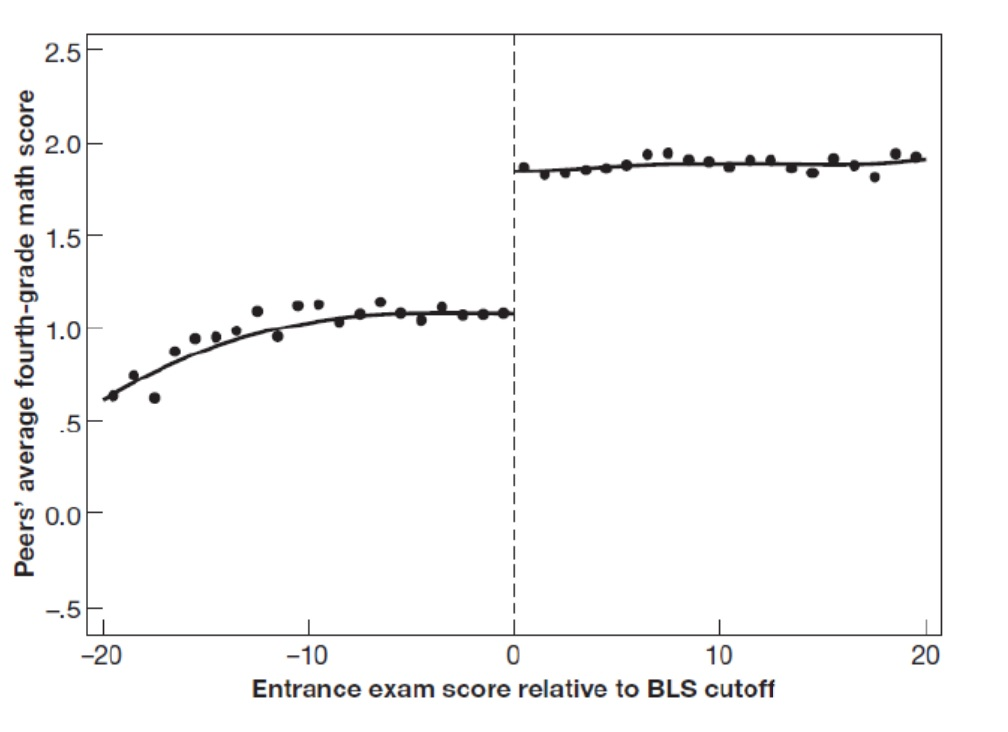
\includegraphics[width=6cm,height=6.5cm,keepaspectratio]{Figure 4.8} 

\column{.45\textwidth}
\begin{itemize}
	\item exam schools induce an experiment in peer quality
	\item applicants who qualify for an exam school attend school with much higher achieving peers
	\item figure shows peer quality around the BLS cut-off
	
\end{itemize}
\end{columns}	
\end{frame}
%---------------------------------------------------
\begin{frame}
\frametitle{Fuzzy RD}
\begin{itemize}
\item in a fuzzy RD research design, applicants who cross a threshold are exposed to a more intense treatment or the probability of being treated changes
\item whereas in a sharp RD research design treatment switches cleanly on or off at the cut-off
\item What is the effect of average schoolmate ability $X_i$ on achievement $Y_i$ of student i?
\end{itemize}
\end{frame}
%---------------------------------------------------
\begin{frame}
\frametitle{Peer Effect}
\begin{itemize}
\item A regression for Boston exam schools would be:
\item $$Y_i = \theta_0 + \theta_1 \={X}_{(i)} + \theta_2X_i + u_i$$
\item the estimated coefficient on peer quality is around 0.25
\item this means that a one standard deviation increase in the ability of middle school peers is associated with a $0.25\sigma$ gain in middle school achievement
\item at the cut-off in our exam school example, peer quality jumps substantially 
\end{itemize}
\end{frame}

%---------------------------------------------------
\begin{frame}
\frametitle{The Peer Effect}
\begin{columns}
\column{.5\textwidth}
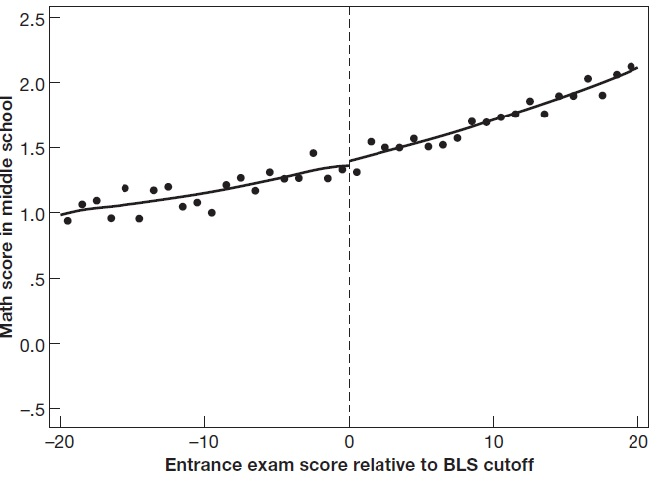
\includegraphics[width=6cm,height=6.5cm,keepaspectratio]{Figure 4.9} 

\column{.45\textwidth}
\begin{itemize}
	\item figure plots seventh and eight grade math scores against exam school admission score for applicants close to cut-off
	\item applicants close to cut-off are exposed to much stronger peer group but this exposure generates no parallel jump in applicant's middle school achievement
	
\end{itemize}
\end{columns}	
\end{frame}
%---------------------------------------------------
\begin{frame}
\frametitle{Peer Quality}
\begin{itemize}
\item in order to figure out how big the jump of middle school grades is, we estimate:
\item $$Y_i = \alpha_0 + \rho D_i + \beta_oR_i + \epsilon_{0i}$$

\item $D_i$ is a dummy indicating applicants who qualify and $R_i$ is the running variable of test scores
\item produces an estimate of $\rho = -.02$ (with standard error .10)
\item the equation is the reduced form for a 2SLS setup where the endogenous variable is the average peer quality $\=X_{(i)}$
\end{itemize}
\end{frame}
%---------------------------------------------------
\begin{frame}
\frametitle{Peer Quality - RD with IV}
\begin{itemize}
\item the first-stage equation would be:
$$ \={X}_{(i)} = \alpha_1 + \phi D_i + \beta_1R_i + \epsilon_1_i$$
\item the second-stage equation can be written as:
$$ Y_i = \alpha_2 + \lambda \^{X}_{(i)} + \beta_2R_i + \epsilon_2_i$$
\item IV-assumption: exam-school qualification has no direct effect on test scores but influences achievement, if at all, through peer quality

\end{itemize}
\end{frame}
%---------------------------------------------------
\begin{frame}
\frametitle{exam schools - Results}
\begin{itemize}
\item the 2SLS estimate of $\lambda$ is -.023 (with standard error of .132), doesn't differ significantly from zero
\item it seems there is no effect of peer quality on school achievement
\item but what about our exclusion restriction?
\end{itemize}
\end{frame}

%---------------------------------------------------
\begin{frame}
\frametitle{exams schools, peer quality and exclusion restriction}
\begin{itemize}
\item exam schools might differ from public schools in other ways: teacher quality, college placement courses, etc. 
\item these differences should all have a positive effect on achievement
\item the OVB associated with 2SLS estimates of exam school peer effect is positive
\item Conclusion: if anything, the estimated peer effect is too large
\end{itemize}
\end{frame}

%---------------------------------------------------
\begin{frame}
\frametitle{In a nutshell}
\begin{itemize}
\item the RD design exploits abrupt changes in treatment status that arise when treatment is determined by a cut-off
\item we need to know the relationship between the running variable and potential outcomes in the absence of treatment
\item finding a perfect control strategy is very hard but we can gain confidence that our strategy is good when RD estimates remain similar as we change details of the RD model
\item a sharp RD is when treatment itself switches on or off at a cut-off whereas in fuzzy designs the probability or intensity of treatment jumps
\item in fuzzy designs a dummy for clearing the cut-off becomes an instrument and the fuzzy design is analyzed by 2SLS
\end{itemize}
\end{frame}



%----------------------------------------------------------------------------------------

\begin{frame}
\Huge{\centerline{Thank you very much for listening}}
\end{frame}

%----------------------------------------------------------------------------------------

\end{document} 